\documentclass[svgnames,11pt]{beamer}
\input{/home/tof/Documents/Cozy/latex-include/preambule_commun.tex}
\input{/home/tof/Documents/Cozy/latex-include/preambule_beamer.tex}
%\usepackage{pgfpages} \setbeameroption{show notes on second screen=left}
\author[]{Christophe Viroulaud}
\title{Découverte du système d'exploitation\\Debian}
\date{\framebox{\textbf{ArchMat 09}}}
%\logo{}
\institute{Première - NSI}

\begin{document}
\begin{frame}
\titlepage
\end{frame}
\begin{frame}
    \frametitle{}

    Les ordinateurs du réseau de l'établissement utilisent le système d'exploitation \textbf{Windows}. Chaque compte utilisateur possède des restrictions afin de préserver l'intégrité du réseau. Ainsi il n'est pas possible d'installer un programme sur une machine du lycée.

\end{frame}
\section{Machine virtuelle}
\begin{frame}
    \frametitle{Machine virtuelle}
    Dans l'établissement certaines restrictions sont posées sur le système d'exploitation \textbf{Windows} des machines. Cependant dans le cadre du cours de NSI, chaque élève dispose d'une \textbf{machine virtuelle}. 
    \begin{aretenir}[]
    Une machine virtuelle est la simulation d'un ordinateur physique. Il est alors possible d'installer un nouveau système d'exploitation sur ce nouvel appareil.
    \end{aretenir}
    Il est alors possible de modifier, tester, se tromper, réinitialiser sans risquer d'interférer avec le réseau pédagogique de l'établissement.
    

\end{frame}
\begin{frame}
    \frametitle{}
La première étape consiste à accéder à sa propre machine virtuelle.
    \begin{activite}
        \begin{enumerate}
            \item Depuis un navigateur, se rendre à l'adresse \url{https://172.17.171.3:8006} .
            \item Remplir le formulaire comme suit:
                  \begin{itemize}
                      \item \emph{utilisateur:} prenom.nom
                      \item \emph{mot de passe:} date de naissance (JJMMAAAA)
                      \item \emph{realm:} Proxmox
                      \item \emph{langue:} Français
                  \end{itemize}
            \item Modifier le mot de passe.
            \item Sur le serveur (bandeau gauche), sélectionner la machine virtuelle avec son nom.
            \item Démarrer la machine (clic-droit ou bouton \emph{démarrer}).
            \item En haut à droite de l'écran, cliquer sur \emph{Console} puis choisir \emph{SPICE}.
        \end{enumerate}
    \end{activite}

\end{frame}
\section{Découvrir Debian}
\begin{frame}
    \frametitle{Découvrir Debian}
    Le système d'exploitation \textbf{Debian (version 10)} est installée sur la machine virtuelle. Debian est une distribution GNU/Linux constituée de logiciels libres et au code source ouvert.
    

\end{frame}
\begin{frame}
    \frametitle{}

    Pour l'instant le système ne possède qu'un compte utilisateur \textbf{nsi} et son mot de passe \textbf{nsi}.
\begin{activite}
    \begin{enumerate}
        \item Ouvrir le système avec le compte \textbf{nsi}.
        \item Cliquer sur \textbf{Activités} en haut à gauche pour découvrir les applications installées. La touche \textbf{Super (Windows sur les claviers)} est un raccourci vers ce menu.
        \item Ouvrir l'application \textbf{Terminal}.
    \end{enumerate}
\end{activite}

\end{frame}
\section{Comptes}
\begin{frame}
    \frametitle{Comptes}
    L'invite de commande du Terminal indique l'utilisateur en cours.
    \begin{center}
    \centering
    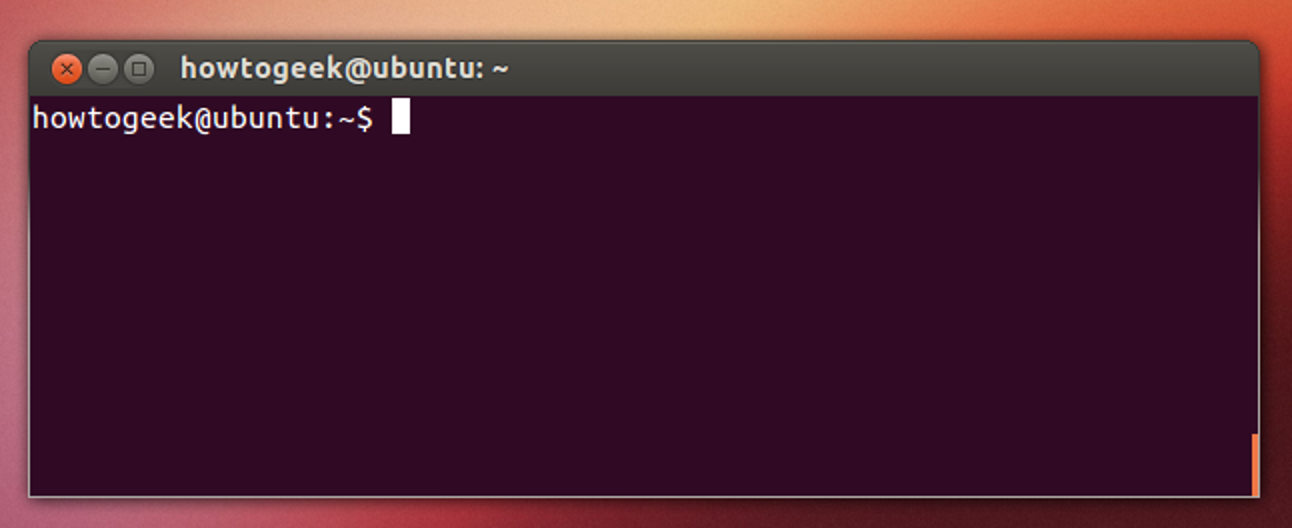
\includegraphics[width=10cm]{ressources/terminal.png}
    \captionof{figure}{\centering L'utilisateur \textbf{howtogeek} est connecté sur l'ordinateur \textbf{ubuntu}.}
    \label{IMG}
    \end{center}

\end{frame}
\begin{frame}
    \frametitle{}

    Les utilisateurs sont répartis dans des groupes qui possèdent certains privilèges. Un utilisateur peut appartenir à plusieurs groupes.
\begin{aretenir}[]
    Le \textbf{super-utilisateur (SU)} possède tous les droits sur la machine. Son identifiant est \textbf{root}. Un utilisateur peut devenir administrateur temporairement. Pour cela il doit appartenir au groupe \textbf{sudo}.
\end{aretenir}

Ainsi, par défaut, l'utilisateur \textbf{nsi} n'a pas tous les privilèges sur la machine. Il est cependant possible d'ajouter cet utilisateur au groupe \textbf{sudo}
\end{frame}
\begin{frame}[fragile]
    \frametitle{}

    \begin{activite}
\begin{enumerate}
\item Dans le Terminal taper la commande. La liste des groupes auxquels appartient l'utilisateur apparaît.
\begin{lstlisting}[language=bash, basicstyle=\ttfamily\small, xleftmargin=2em, xrightmargin=2em]
groups
\end{lstlisting}
\item Pour devenir super-utilisateur, taper la commande ci-après. Le mot de passe est également \textbf{nsi}.
\begin{lstlisting}[language=bash, basicstyle=\ttfamily\small, xleftmargin=2em, xrightmargin=2em]
su -
\end{lstlisting}
On peut remarquer que le nom de l'utilisateur affiché sur la ligne de commande a changé.
\item Modifier le mot de passe du super-utilisateur. \textbf{Il est impératif de ne pas perdre ce mot de passe!}
\begin{lstlisting}[language=bash, basicstyle=\ttfamily\small, xleftmargin=2em, xrightmargin=2em]
passwd
\end{lstlisting}
\end{enumerate}
\end{activite}

\end{frame}
\begin{frame}
    \frametitle{}

    \begin{framed}
        \centering \textbf{Ai-je précisé qu'il fallait impérativement ne pas oublier ce mot de passe?}
    \end{framed}

\end{frame}
\begin{frame}[fragile]
    \frametitle{}

\begin{activite}
\begin{enumerate}
\item Créer un compte personnel. Il faut remplacer \emph{mon\_identifiant}. \textbf{Bien retenir le mot de passe!} Le questionnaire qui est posé ensuite est facultatif.
\begin{lstlisting}[language=bash, basicstyle=\ttfamily\small, xleftmargin=2em, xrightmargin=2em]
# remplacer mon_identifiant par un identifiant personnel
adduser mon_identifiant
\end{lstlisting}
\item Ajouter le nouveau compte au groupe \emph{sudo}.
\begin{lstlisting}[language=bash, basicstyle=\ttfamily\small, xleftmargin=2em, xrightmargin=2em]
usermod -aG sudo mon_identifiant
\end{lstlisting}
\item Vérifier les groupes auxquels appartient le nouveau compte.
\begin{lstlisting}[language=bash, basicstyle=\ttfamily\small, xleftmargin=2em, xrightmargin=2em]
groups mon_identifiant
\end{lstlisting}
\item Sortir du mode super-utilisateur.
\begin{lstlisting}[language=bash, basicstyle=\ttfamily\small, xleftmargin=2em, xrightmargin=2em]
exit
\end{lstlisting}
\end{enumerate}
\end{activite}

\end{frame}
\begin{frame}
    \frametitle{}

    Il existe maintenant 3 comptes utilisateurs:
    \begin{itemize}
        \item le super-utilisateur \textbf{root},
        \item l'utilisateur \textbf{nsi},
        \item le nouvel utilisateur \textbf{mon\_identifiant}.
    \end{itemize}

    Le super-utilisateur possède tous les privilèges. Les deux autres comptes appartiennent au groupe \textbf{sudo}: ils peuvent donc devenir super-utilisateur temporairement.
\end{frame}
\begin{frame}[fragile]
    \frametitle{}

\begin{activite}
\begin{enumerate}
\item Redémarrer le système.
\item Se connecter avec le nouveau compte.
\item Supprimer le compte \textbf{nsi}.
\begin{lstlisting}[language=bash, basicstyle=\ttfamily\small, xleftmargin=1em, xrightmargin=0em]
# L'ajout du mot sudo exécute la commande en mode super-utilisateur.
sudo deluser --remove-home nsi
# On utilise ici le mot de passe du compte personnel
\end{lstlisting}
\end{enumerate}
\end{activite}   

\end{frame}
\begin{frame}[fragile]
    \frametitle{}
    Sur le réseau chaque machine peut être repéré par son \textbf{nom d'hôte (hostname)}.
\begin{activite}
    Remplacer le nom de la machine:
    \begin{itemize}
        \item Ouvrir le fichier hostname
\begin{lstlisting}[language=bash, basicstyle=\ttfamily\small, xleftmargin=1em, xrightmargin=1em]
sudo nano /etc/hostname
\end{lstlisting}
\item Remplacer le nom de la machine.
\item Enregistrer avec le raccourci \textbf{Ctrl+O}.
\item Sortir de l'éditeur \textbf{nano}: \textbf{Ctrl+X}.
    \end{itemize}
\end{activite}

\end{frame}
\section{Mise à jour et installation d'applications}
\subsection{Connexion au web}
\begin{frame}
    \frametitle{Mise à jour - Connexion au web}

    \begin{aretenir}[Observation]
Le fonctionnement des ordinateurs dans le lycée est différent de celui d'une machine personnelle. Pour se connecter au web, un particulier ouvrira son navigateur\dots et c'est tout.\\
Dans le lycée les machines virtuelles sont isolées dans une \emph{bulle}. Pour se connecter au web, il faut établir un tunnel vers l'extérieur: c'est le rôle de l'application \textbf{alcasar}.
    \end{aretenir}

\end{frame}
\begin{frame}
    \frametitle{}

    \begin{activite}
        \begin{enumerate}
            \item Ouvrir Firefox.
            \item Ouvrir la page \url{http://alcasar.localdomain}
            \item Entrer les identifiants. Il s'agit des mêmes que le serveur \emph{Proxmox} \textbf{lors de la première connexion}. Il faut donc utiliser la date de naissance pour mot de passe.
            \item Modifier le mot de passe. 
            
        \end{enumerate}
        \end{activite}
        \begin{framed}
            \centering \textbf{Je ne me rappelle plus si je vous ai déjà dit de ne pas oublier ce mot de passe.}
        \end{framed}
\end{frame}
\begin{frame}
    \frametitle{}

    \begin{aretenir}[Observation]
    Tant que la fenêtre \textbf{alcasar} reste ouverte, la machine peut accéder au web;
    \end{aretenir}

\end{frame}
\subsection{Aptitude}
\begin{frame}
    \frametitle{Aptitude}

    Il existe une logithèque qui permet d'installer des applications. Cet outil est accessible en mode graphique: \textbf{logiciels}. Cependant il est également possible de réaliser les manipulations avec le Terminal. Sur Debian les logiciels sont installés via un \textbf{dépôt} officiel. Ce principe est similaire aux boutiques d'application (Play store\dots). Cette méthode permet de limiter la circulation de virus, malwares\dots L'application \textbf{apt} permet de gérer les paquets installés.

\end{frame}
\begin{frame}[fragile]
    \frametitle{}
\begin{activite}
\begin{enumerate}
\item Mettre à jour la liste des paquets. Cette étape n'installe rien mais compare seulement les versions des applications de la machine à celles du dépôt.
\begin{lstlisting}[language=bash, basicstyle=\ttfamily\small, xleftmargin=2em, xrightmargin=2em]
sudo apt update
\end{lstlisting}
\item Mettre à jour les paquets. Cette étape installe les nouvelles versions des logiciels déjà installés.
\begin{lstlisting}[language=bash, basicstyle=\ttfamily\small, xleftmargin=2em, xrightmargin=2em]
sudo apt upgrade
\end{lstlisting}
\item Vérifier la présence d'une application.
\begin{lstlisting}[language=bash, basicstyle=\ttfamily\small, xleftmargin=2em, xrightmargin=2em]
# vérifie si le logiciel extrepo est installé
apt policy extrepo
\end{lstlisting}
\item Installer une application. Nous installons \textbf{extrepo} qui nous sera utile ensuite.
\begin{lstlisting}[language=bash, basicstyle=\ttfamily\small, xleftmargin=2em, xrightmargin=2em]
sudo apt install extrepo
\end{lstlisting}
\end{enumerate}
\end{activite}

\end{frame}
\subsection{Dépôt non-officiel}
\begin{frame}
    \frametitle{Dépôt non-officiel}

    Certaines applications ne sont pas présentes dans les dépôts officiels. Même s'il faut rester prudent, il est possible d'ajouter de nouveaux dépôts.

\end{frame}
\begin{frame}[fragile]
    \frametitle{}
L'application \textbf{extrepo} précédemment installée permet d'activer facilement des dépôts non-officiels.
\begin{activite}
\begin{enumerate}
\item Activer le dépôt du logiciel \textbf{vscodium}.
\begin{lstlisting}[language=bash , basicstyle=\ttfamily\small, xleftmargin=2em, xrightmargin=2em]
sudo extrepo enable vscodium
\end{lstlisting}
\item Installer le logiciel \textbf{vscodium}
\begin{lstlisting}[language=bash , basicstyle=\ttfamily\small, xleftmargin=2em, xrightmargin=2em]
sudo apt install vscodium
\end{lstlisting} 
\item \emph{Pour les plus avancés:} Découvrir \textbf{vscodium} et installer des extensions en s'aidant du guide sur le lien suivant: \url{https://tinyurl.com/vscodium}
\end{enumerate}
\end{activite}

\end{frame}
\end{document}